% Christoffel Symbol Computation Flowchart
% Pedagogical visualization showing step-by-step computation process
% For Chapter 1: Mathematical Preliminaries

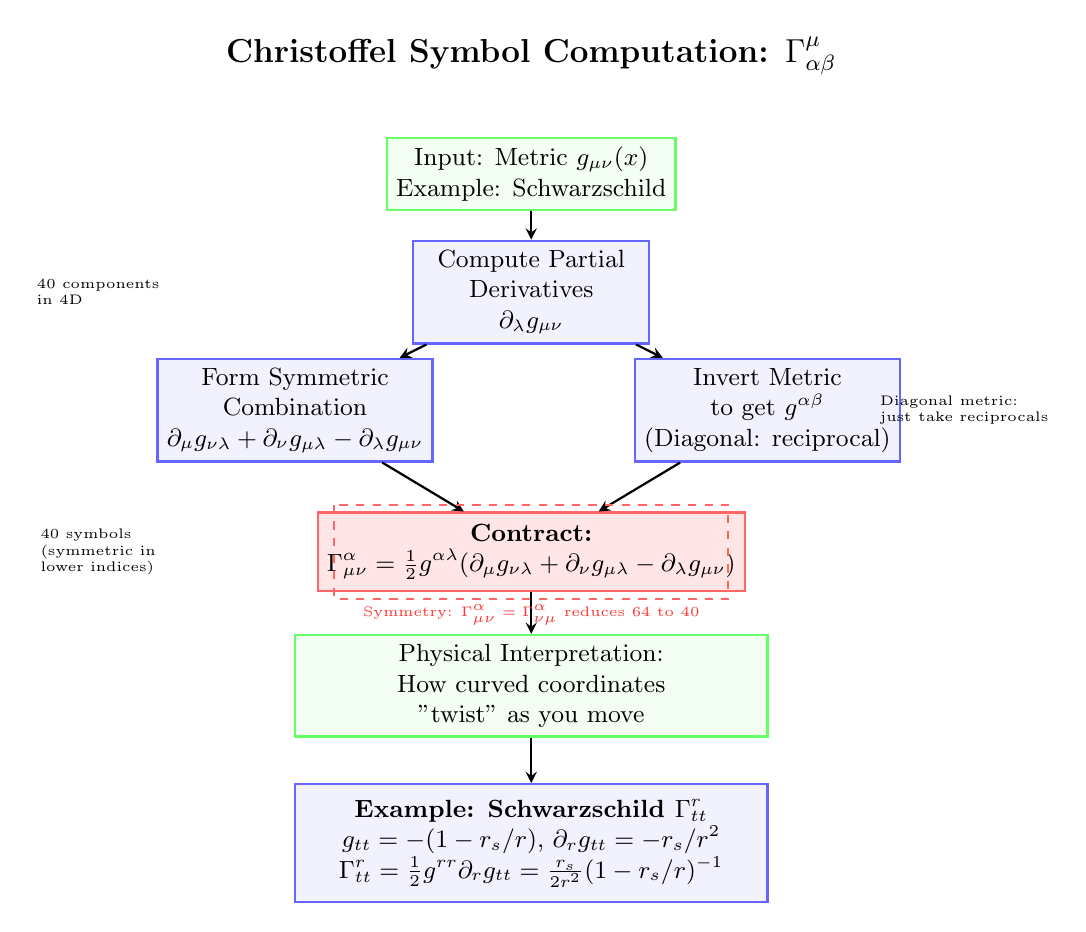
\begin{tikzpicture}[
    node distance=1.2cm and 2cm,
    box/.style={rectangle, draw=blue!60, fill=blue!5, thick, minimum width=3cm, minimum height=0.8cm, align=center, font=\small},
    databox/.style={rectangle, draw=green!60, fill=green!5, thick, minimum width=3cm, minimum height=0.8cm, align=center, font=\small},
    resultbox/.style={rectangle, draw=red!60, fill=red!10, thick, minimum width=3cm, minimum height=1cm, align=center, font=\small\bfseries},
    arrow/.style={->, >=stealth, thick}
]

% Title
\node[font=\large\bfseries] at (0,5.5) {Christoffel Symbol Computation: $\Gamma^\mu_{\alpha\beta}$};

% Step 1: Input metric
\node[databox] (metric) at (0,4) {Input: Metric $g_{\mu\nu}(x)$\\Example: Schwarzschild};

% Step 2: Compute derivatives
\node[box] (deriv) at (0,2.5) {Compute Partial\\Derivatives\\$\partial_\lambda g_{\mu\nu}$};

% Step 3: Form symmetric combination
\node[box] (symm) at (-3,1) {Form Symmetric\\Combination\\$\partial_\mu g_{\nu\lambda} + \partial_\nu g_{\mu\lambda} - \partial_\lambda g_{\mu\nu}$};

% Step 4: Invert metric
\node[box] (invert) at (3,1) {Invert Metric\\to get $g^{\alpha\beta}$\\(Diagonal: reciprocal)};

% Step 5: Contract
\node[resultbox] (result) at (0,-0.8) {Contract:\\$\Gamma^\alpha_{\mu\nu} = \frac{1}{2}g^{\alpha\lambda}(\partial_\mu g_{\nu\lambda} + \partial_\nu g_{\mu\lambda} - \partial_\lambda g_{\mu\nu})$};

% Step 6: Physical interpretation
\node[databox, minimum width=6cm] (phys) at (0,-2.5) {Physical Interpretation:\\How curved coordinates\\"twist" as you move};

% Example calculation box
\node[box, minimum width=6cm, minimum height=1.5cm] (example) at (0,-4.5) {
    \textbf{Example: Schwarzschild $\Gamma^r_{tt}$}\\
    $g_{tt} = -(1-r_s/r)$, $\partial_r g_{tt} = -r_s/r^2$\\
    $\Gamma^r_{tt} = \frac{1}{2}g^{rr}\partial_r g_{tt} = \frac{r_s}{2r^2}(1-r_s/r)^{-1}$
};

% Arrows
\draw[arrow] (metric) -- (deriv);
\draw[arrow] (deriv) -- (symm);
\draw[arrow] (deriv) -- (invert);
\draw[arrow] (symm) -- (result);
\draw[arrow] (invert) -- (result);
\draw[arrow] (result) -- (phys);
\draw[arrow] (phys) -- (example);

% Annotations
\node[font=\tiny, align=left] at (-5.5,2.5) {40 components\\in 4D};
\node[font=\tiny, align=left] at (5.5,1) {Diagonal metric:\\just take reciprocals};
\node[font=\tiny, align=left] at (-5.5,-0.8) {40 symbols\\(symmetric in\\lower indices)};

% Symmetry note
\draw[dashed, thick, red!60] (-2.5,-0.2) rectangle (2.5,-1.4);
\node[font=\tiny, text=red!80] at (0,-1.6) {Symmetry: $\Gamma^\alpha_{\mu\nu} = \Gamma^\alpha_{\nu\mu}$ reduces 64 to 40};

\end{tikzpicture}
